\section{Project Constraints}

Project constraints can be defined as all the limitations that curb the action of the project team and restrict project’s outcome. It is necessary to define them with caution and common sense to avoid determining constraints that lead us to an impossible project, especially in terms of cost, time and resources. They can be internal limitations (scope, budget, etc.) or external limitations (environmental impact, stakeholders, government regulations, etc.)

In this project, we have decided to adopt a classification consisting on six groups \cite{workfront2017} where constraints can be clearly interpreted and organised.

\begin{figure}[H]
	\centering
	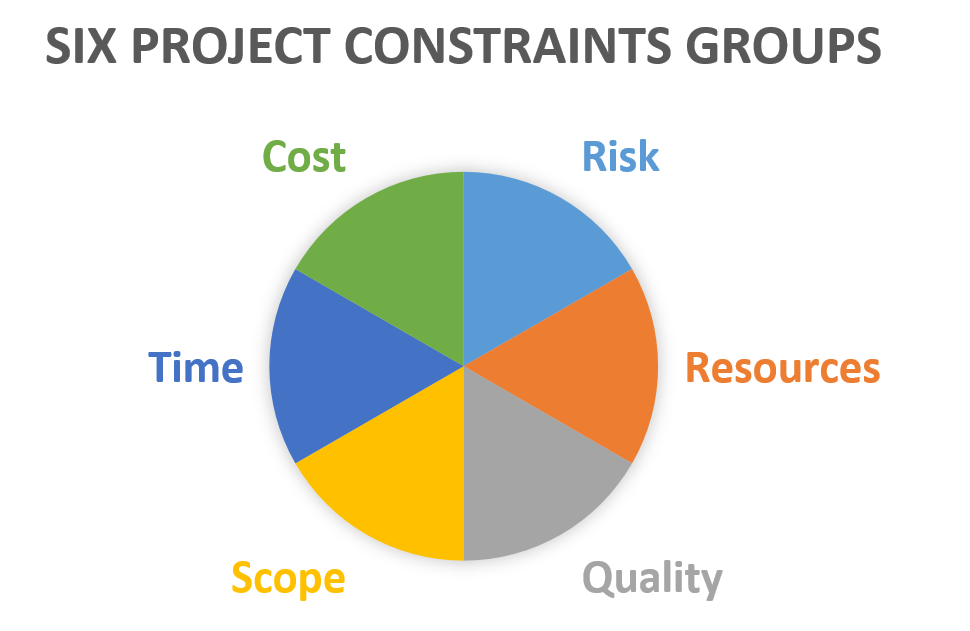
\includegraphics[width=0.65\linewidth]{./images/constraints}
	\caption[The 6 Project Constraints]{The 6 Project Constraints \cite{workfront2017}.}
	\label{fig:constraints}
\end{figure}

It is important to highlight that groups are interrelated in a way that if one of them changes, then, one or more of the others will be affected.

\textbf{Scope}

\begin{itemize}
	
	\item \textbf{State of the art:} The starting point of the project has to be based on a study of the optical and radar cutting-edge technologies, not on outdated ones.
	
	\item \textbf{Technologies selection:} The technologies to be developed must be the most promising systems to profit Earth Observation, air composition and terrain analysis.
	
	\item \textbf{Technologies improvement:} The project is required to enhance the selected technologies in order to accomplish the European Commission requirements.
	
	\item \textbf{Final design:} The resulting design has to be a compact product which contains the chosen sensors, sharing a data collection software.
	
\end{itemize}

\textbf{Time}

\begin{itemize}
	
	\item \textbf{Deadlines:} All deliverables have to be completed in their scheduled dates:
	
	\begin{itemize}
		
		\item \textbf{10/09/2018 – } Kick-Off meeting 
		
		\item \textbf{05/10/2018 – } Project Management, Business and Communication Plans
		
		\item \textbf{28/12/2018 – } State of the Art completion
		
		\item \textbf{14/06/2019 – } Payload preliminary report
		
		\item \textbf{06/09/2019 – } Modular system preliminary design
		
		\item \textbf{29/11/2019 – } Interaction platform preliminary design
		
		\item \textbf{15/05/2020 – } Mid-term project report
		
		\item \textbf{12/06/2020 – } Payload final design
		
		\item \textbf{04/09/2020 – } Modular system final design 
		
		\item \textbf{27/11/2020 – } Interaction platform final design
		
		\item \textbf{16/04/2021 – } Prototype manufacturing
		
		\item \textbf{09/07/2021 – } Individual systems testing 
		
		\item \textbf{29/10/2021 – } Full system testing
		
		\item \textbf{21/01/2022 – } Project completion
		
	\end{itemize}
	
	\item \textbf{Schedule:}
	
	\begin{itemize}
		
		\item \textbf{Follow Gantt chart organization:} Tasks must be developed in the initially accorded order, avoiding undesired overlapping or delays and bringing the requirements of each task to their completion.
		
	\end{itemize}
	

\end{itemize}

\textbf{Cost}

\begin{itemize}
	
	\item \textbf{Budget:}
	
	\begin{itemize}
		
		\item All the incomes have to come from the European Commission.
		
		\item The project cannot exceed the quantity of 4 million euros.
		
		\item The money distribution must be done as it was described in the estimated budget.
		
	\end{itemize}

\end{itemize}

\textbf{Resources}

\begin{itemize}
	
	\item \textbf{Facilities:} No tasks will be planned without the certainty that the team (or a stakeholder) has the necessary facilities to complete it.
	
	\item \textbf{Human resources:} All the labour hours made by the staff in charge of the project must be justified. Every task will have assigned a different number of workers depending on the difficulty and duration.
	
	\item \textbf{Infrastructures:} The work to be done by the team is restricted by the capacity, limitations and efficiency of the owned infrastructures.
	
	\item \textbf{Procurement:} Goods and services will be obtained following optimized processes to achieve minimum cost while at the same time requirements are properly fulfilled.
	
	\item \textbf{Technical constraints:} The developement of the new technologies that the product will use will be restricted by technical, physical and scientific limitations.
	
	
\end{itemize}

\textbf{Risks}

\begin{itemize}
	
	\item \textbf{Risk tolerance:} The amount of risk that the project must handle has to be low. It means that if some risky event has a low probability to happen, the impact can be low or moderate. On the other hand, if the event has a high probability to happen, the impact must be low.
	
	\item \textbf{Actions:} When some risk becomes a real problem for the project, the necessary measures have to be taken. These must affect as little as possible to the other constraints, such as cost or time.
	
\end{itemize}

\textbf{Quality}

\begin{itemize}
	
	\item \textbf{Legal constraints:} All the systems developments and tests must be carried out under the corresponding standards. 
	
	\item \textbf{Methodology:} The project must be developed following a methodology based on the use of state of the art technologies, research and improvement of the current capabilities of the earth observation systems.
	
	\item \textbf{Organization:} To obtain the required quality, communication between departments, communication with stakeholders, and the use of project management software assistance is a must.
	
	\item \textbf{Stakeholders’ expectations:} External constraints imposed by stakeholders must be accounted in the project. In addition, the agreements with each of them must be accomplished.
	
	\item \textbf{Customer satisfaction:} The final product must fulfil the stablished requirements to obtain the customer satisfaction.
	
\end{itemize}